\documentclass[11pt]{beamer}

\usepackage{url}
\usepackage{tikz}
\author{Armijn Hemel\\Tjaldur Software Governance Solutions}
\title{}
\date{April 5, 2012}

\begin{document}

\setlength{\parskip}{4pt}

\frame{\titlepage}

\frame{
\frametitle{About Armijn}

\begin{itemize}
\item using Open Source software since 1994
\item MSc Computer Science from Utrecht University (The Netherlands)
\item core team \url{gpl-violations.org} since 2005
%\item ex-board member at NLUUG (\url{http://www.nluug.nl/})
%\item sysadmin, developer and consultant at Loohuis Consulting (2006 - May 2011)
\item owner Tjaldur Software Governance Solutions since May 2011
\end{itemize}
}

\frame{
\frametitle{Subjects}

\begin{itemize}
\item very brief overview of license violations
\item problems in binary code clone detection
\item open questions in binary code clone detection
\end{itemize}
}

\frame{
\frametitle{License enforcement}

\begin{itemize}
\item Europe (Germany, France) \& USA
\item focus is on GPLv2 and LGPLv2/2.1
\item done by companies (Nokia, Red Hat) and individual developers and projects (Harald Welte, BusyBox, XviD, etc.)
\end{itemize}

It is about copyright, not about patents!
}

\frame{
\frametitle{gpl-violations.org}
Founded in 2004 by Harald Welte (copyright holder in the Linux kernel) to take on GPL license violations by:

\begin{itemize}
\item education
\item documentation
\item legal action
\end{itemize}

I have been active with \url{gpl-violations.org} since 2005.

So far we've had several hundred cases (most of them settled) and fixed many more using informal pressure.
}

\frame{
\frametitle{How gpl-violations.org works}

\begin{enumerate}
\item we get a report via private email, public mailing list, chat, rumours, SMS, or our own research
\item if there is reasonable doubt about compliance of a device we do a test purchase to confirm the violation
\item if we confirm a violation we send a ``cease and desist''
\end{enumerate}

There are many false reports: a lot of people don't understand the license(s).

Our main focus is on consumer electronics (one of the biggest markets out there).
}

\frame{
\frametitle{Consumer electronics: the truth}
Almost everything is purchased. Making everything yourself is commercial suicide:

\begin{itemize}
\item extremely thin margins
\item cut throat competition
\item quality is less important than price
\item (ultra) short term thinking: companies don't know if they will still be in business in 6 months from now
\item ``cowboys''
\end{itemize}

It's like Nike: don't do any production, just marketing and sales.

In my experience typically more than 95\% (or more) is reuse of open source software (with/without modifications)
}

\frame{
\frametitle{}
  \begin{tikzpicture}[remember picture,overlay]
    %\node[yshift=0.3cm] at (current page.center)
    \node[yshift=-0.3cm] at (current page.center)
    {
      \pgfimage[width=\linewidth]{alibaba}
    };
  \end{tikzpicture}
}

\frame{
\frametitle{Problem source: supply chain}
License violations are often a direct result of a mistake made in the supply chain:

\begin{itemize}
\item chipset vendors
\item board makers
\item SDK (``Software Development Kit'') vendor
\item reference design makers
\item product customizers
\item ``labellers''
\end{itemize}

The ``labellers'' get sued and are responsible, even though they add/modify the least amount of code!
}

\frame{
\frametitle{Industry responses to enforcement}

\begin{itemize}
\item extreme levels of frustration (problem doesn't go away by throwing money at it)
\item they don't care about licenses, they just want to sell a product. Licenses are a nuisance that needs to be dealt with.
\item a single enforcement case will make no change to the market (it is too big: a single company getting in trouble is not significant to push for change)
\item no ill will. Companies want to fix it and there is a need for tools (cheap, or free) to do ``due dilligence''
\end{itemize}
}

\frame{
\frametitle{Tools}
Apart from the obvious ``industry standard'' tools that solve some problems Tjaldur Software Governance Solutions has worked on tools to help solving specific problems in this field.

Goal: let companies do checks themselves, increasing quality and lowering costs.

\begin{itemize}
\item Binary Analysis Tool (Apache 2 license, freemium model)
\item license scanning tools (leveraging existing tools like Ninka and FOSSology)
\item long term: build system integration (preliminary work has been done)
\end{itemize}
}

\frame{
\frametitle{Binary Analysis Tool}

\begin{itemize}
\item generic extensible pluggable framework for analysing binaries
\item binary code clone detection using string comparisons: first extract string constants from the binary, compare it with a large database of data extracted from source code, finally assign a score to packages based on matches
\end{itemize}

Demo later.
}

\frame{
\frametitle{Binary code clone detection}

``Finding Software License Violations Through Binary Code Clone Detection'' (Mining Software Repositories 2011) - some results have been integrated into Binary Analysis Tool

Very simple, but very effective, method using comparison of string constants:

\begin{enumerate}
\item extract strings from source code using \texttt{xgettext}
\item store strings in database, using some additional information (file name, package name, version, programming language)
\item extract strings from a binary (different methods per binary to decrease false positives)
\item use statistics to compute a score
\end{enumerate}
}

\frame{

\frametitle{Computing a score for a package}

\begin{enumerate}
\item if the string is unique add the length of the string to the score
\item if it is not unique, decrease the score exponentially depending on the amount of packages it is in
\item determine in which package the string is. In case of internal cloning assign a string (and its score) to a package using a ``battle royale''
\end{enumerate}
}

\frame{
\frametitle{Weeding out false positives}

Extracting strings from binaries in a smart way:

\begin{itemize}
\item only use \texttt{data} and \texttt{rodata} sections from ELF binary, if available
\item extract string constants from Java binaries using \texttt{jcf-dump --print-constants}
\item extract string constants from Dalvik (Android) binaries using Dedexer
\end{itemize}

This reduces the amount of false positives and increases fidelity.

Not done (yet):

\begin{itemize}
\item bFLT (ucLinux, not used much anymore, largely irrelevant)
\item .NET
\end{itemize}
}

\frame{
\frametitle{Causes of false positives and false negatives}
\begin{itemize}
\item \texttt{xgettext} is not always correct (can't deal with special characters like NUL)
\item some strings are defined using escaping in one package and cloned without escaping in another
\item generated source code
\item I make a strong distinction between language families because code reuse between packages in two language families is unlikely, but this makes it hard when code in another language is embedded (especially an issue for .NET)
\item hard to decide where to distinguish between systems where it is unlikely that code is being reused (Linux kernel and desktop will have extremely little overlap)
\end{itemize}
}

\frame{

\frametitle{Seeing BAT in action}

\begin{itemize}
\item running a full analysis on a simple firmware
\item new viewer (not released yet, still quite bad performance in some cases), to view results of the scan
\end{itemize}
}

\frame{

\frametitle{Using information from ELF dynamic symbol table}
Dynamically linked ELF binaries have a lot of information recorded in the binary, including function names:

\begin{itemize}
\item \texttt{readelf -W --dyn-syms}
\item filter out everything that is not a function
\item filter out everything that is not local, but is linked at runtime (indicated using \texttt{UND})
\end{itemize}

Using a similar method as string ranking you can do function name ranking:

\begin{itemize}
\item use \texttt{ctags} to extract function names from source code
\item record function names in database, with meta information
\item match function names from binary with strings from database
\end{itemize}

Unfortunately: no demo, since this is still very early days (few days old) and not very efficient (yet). Test runs with some experimental data are very promising though.
}

\frame{
\frametitle{Defeating obfuscation}
Few companies hide violations on purpose. For each company there comes a point when they want to give up on obfuscation.

\begin{itemize}
\item verbatim string matches are easy to work around, but there could still be enough partial evidence (substring matches)
\item changing names of function names has additional risks: you are changing the API of programs/libraries
\end{itemize}

The biggest cost: testing and making sure that things continue to work as planned.

Next steps: generate signatures from compiled code.

Also, avoiding detection means taking many more steps:

\begin{itemize}
\item scrubbing (network)
\item hiding services
\item locking down machines (network, services, hardware via serial port/JTAG)
\end{itemize}
}

\frame{
\frametitle{Open questions/problems about binary code clone detection}

\begin{itemize}
\item detecting obfuscated code in binaries (when basic string comparisons simply aren't enough)
\item detecting language embedding (interpreters, DSLs) in binaries (if they have been compiled)
\item correlating binary code and source code (solved for source to binary using tracing, not from binary to source side)
\item complete provenance of binary and source code files, down to the level of single commits (example: individual Git commits) because snapshots from DVCS (like Git) are rapidly replacing normal releases
\item reducing false positives in detection: false claims can lead to counter lawsuits, with significant risks
\end{itemize}
}

\frame{
\frametitle{Analyzing build processes}
``What Goes into an Executable? Identifying a Binary's Sources by Tracing Build Processes'' (sent to WCRE 2011 and ICSE 2012, unfortunatey rejected)

Simple method:

\begin{itemize}
\item forget about static analysis
\item use \textit{tracing} to instrument the build process
\item postprocess output from trace and record dependencies between artefacts and inputs
\item get information about relevant inputs (license, copyrights, security information, \dots)
\end{itemize}

I'm preparing more tooling that implements this (rough prototypes exist).
}

\frame{
\frametitle{Example: \texttt{opkg}}
\texttt{opkg} is a package manager that is used on embedded Linux distributions.

Question: given a binary of \texttt{opkg}, what license(s) can it be distributed
under?
}

\frame{
\frametitle{GPLv2? GPLv2+? GPLv3+?}
\texttt{opkg} has a \texttt{COPYING} file containing the text of GPLv2.

All source code files in \texttt{opkg} are GPLv2+ \textbf{except} \texttt{libopkg/sha256.c} and \texttt{libopkg/sha256.h} whi
ch are GPLv3+!

These files are not always included, but they are most of the time. The \texttt{configure} script has a switch:

\texttt{\\   --enable-sha256         Enable sha256sum check [default=yes]\\}

Correct answer: it depends and more information about the \texttt{composition} of the binary is needed.
}

\frame{
\frametitle{Tracing software use case: FFmpeg}
\texttt{FFmpeg} is a mix of GPLv2+ and LGPLv2.1+ licensed code. The \texttt{configure} script has an option to only use the LGPLv2.1+ sources for a build.

With our approach we found that some GPLv2+ code was \textit{always} included in \texttt{libavfilter}.

The offending code was in \texttt{libavfilter/x86/gradfun.c}, licensed under the GPLv2+.

This was not trivial to find out from the \texttt{FFmpeg} build scripts.

\texttt{FFmpeg} fixed it within hours after being informed.
}

\begin{frame}[fragile]
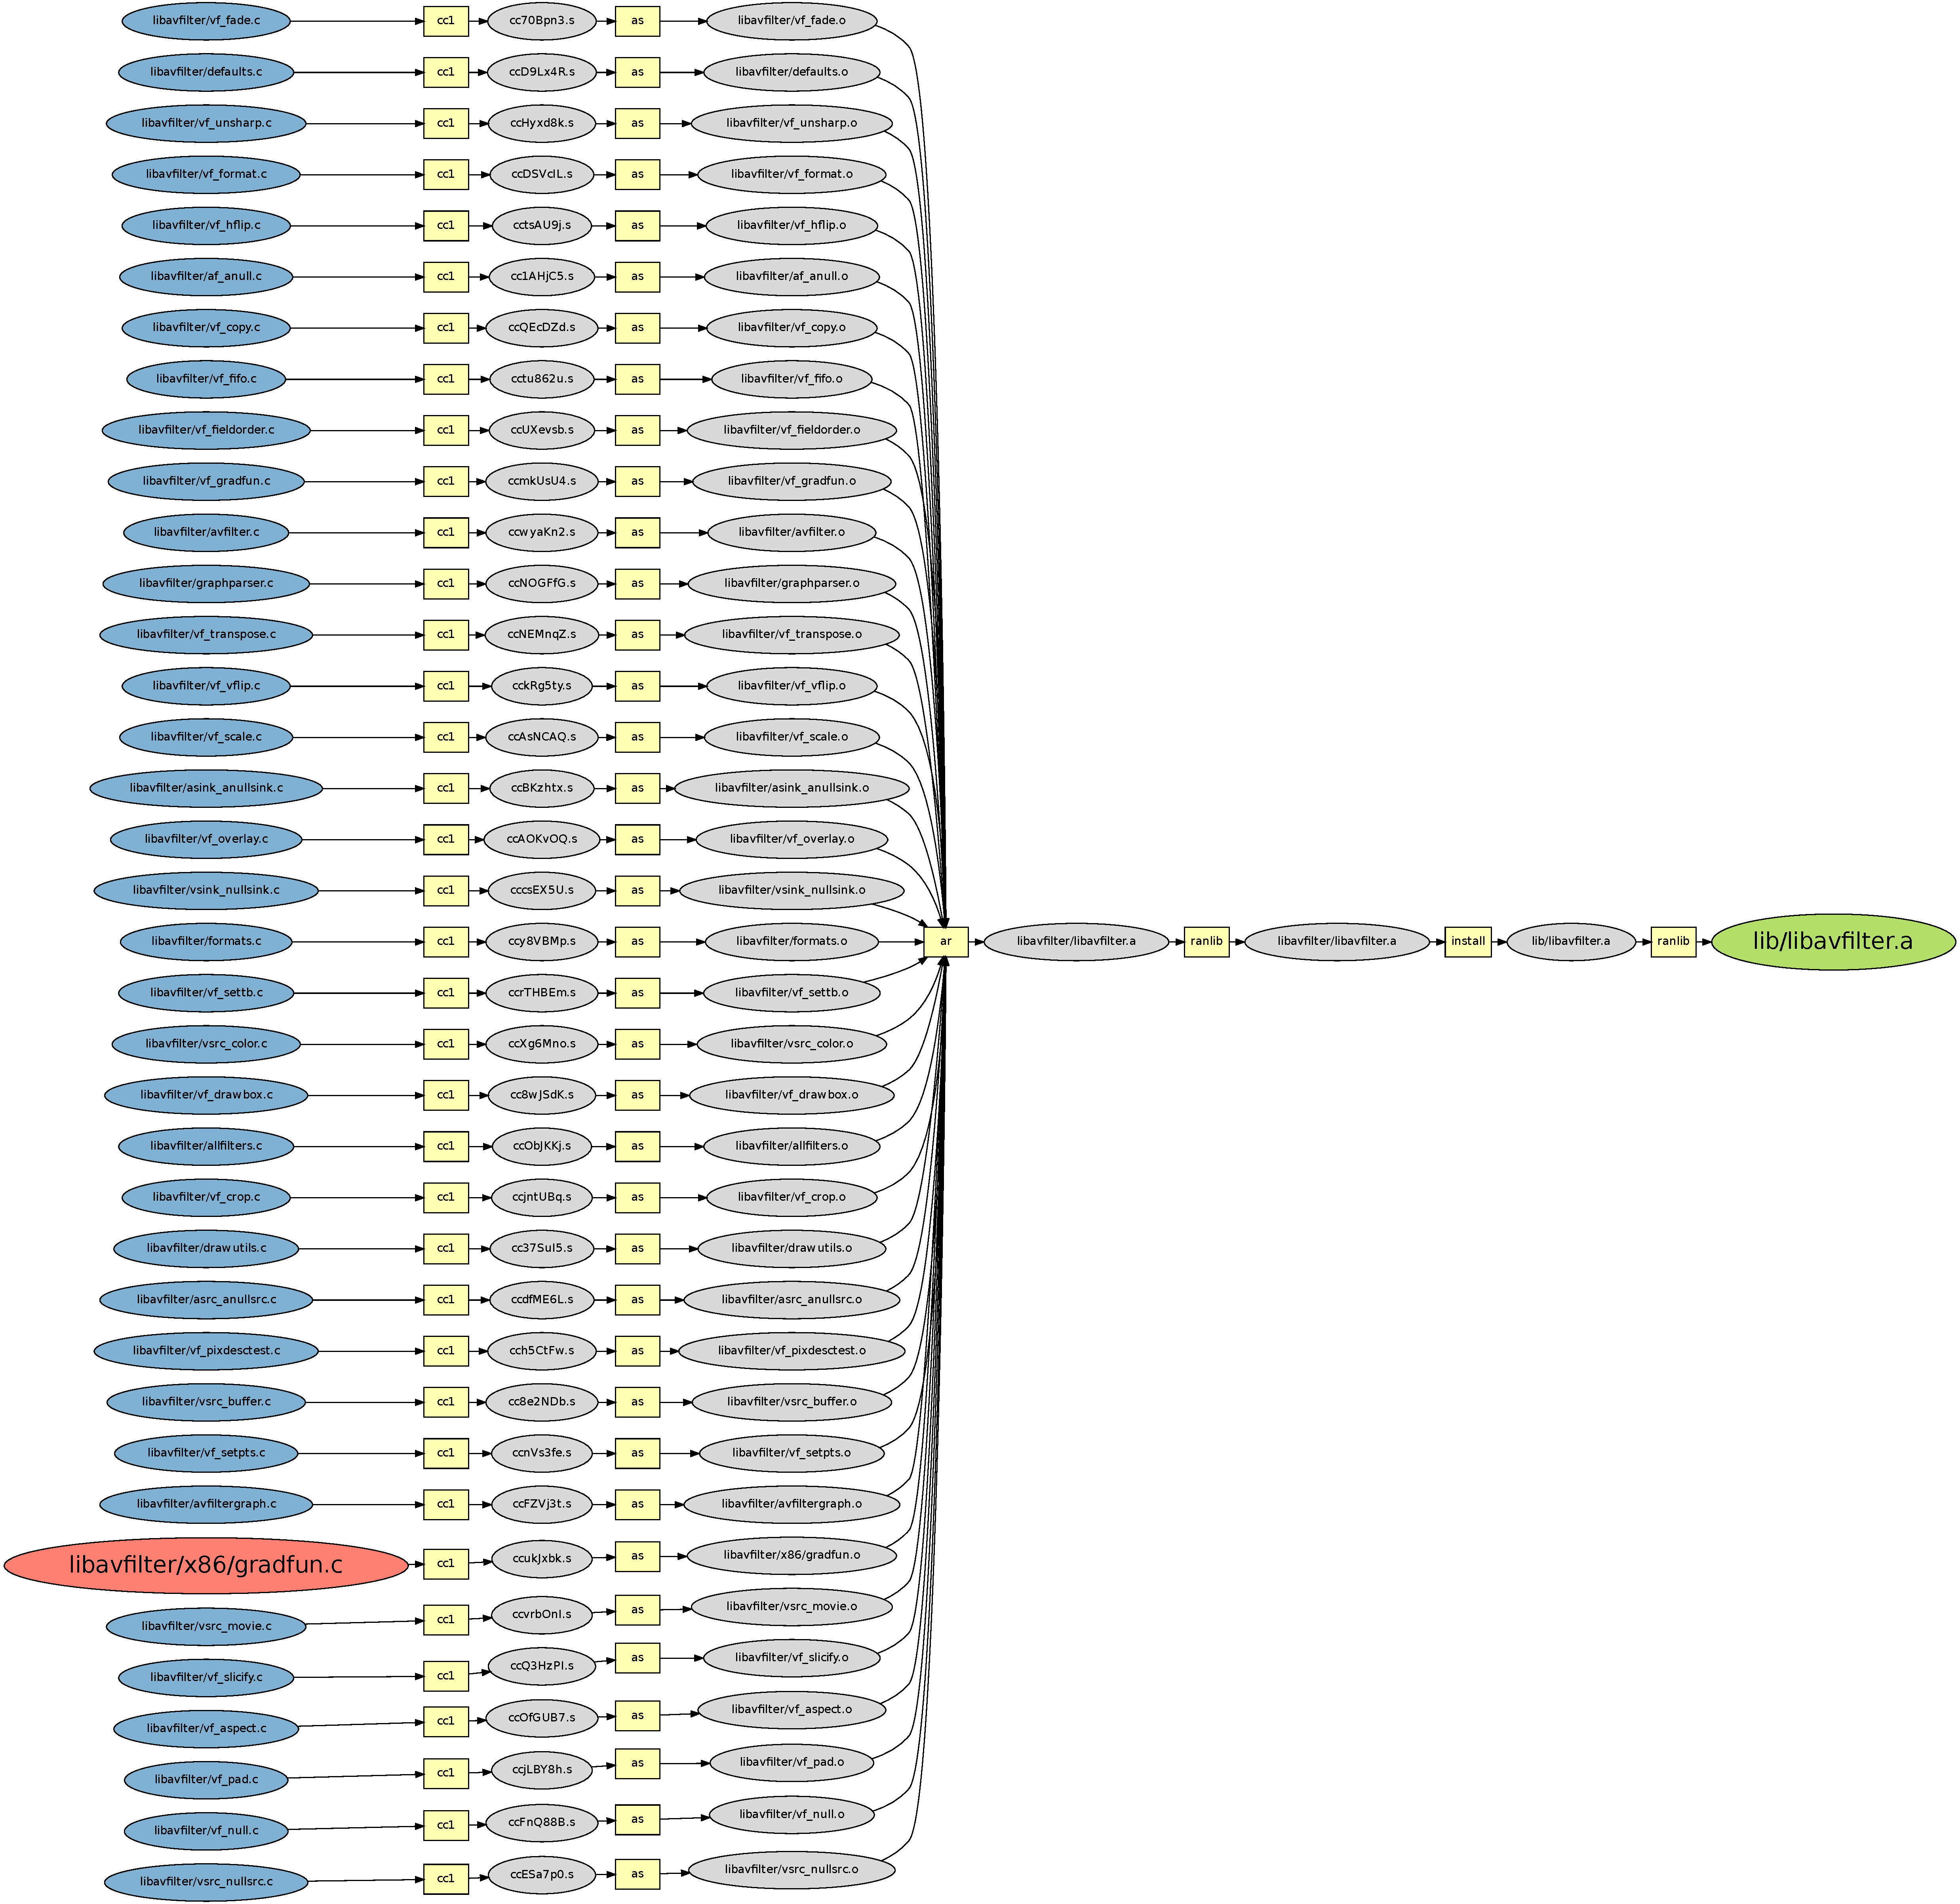
\includegraphics[width=0.9\columnwidth]{ffmpeg_no_gpl_libavfilter_crop}
\end{frame}

\frame{
\frametitle{Runtime analysis}
Most interesting is analysis at runtime:

\begin{itemize}
\item libraries at buildtime might be different to runtime (dynamically linked executables)
\item there might be dependencies that are undetectable using static analysis or at buildtime (\texttt{dynload()}, web services, \dots)
\end{itemize}
}

\frame{
\frametitle{Q \& A}
}

\end{document}
